\documentclass{mrl}
\usepackage{amsthm,amsmath}
\usepackage{listings}
\lstset{basicstyle=\ttfamily\footnotesize,breaklines=true}
\usepackage{hyperref}
\usepackage[utf8]{inputenc}
\usepackage{graphicx}
\usepackage{enumerate}
\begin{document}
\begin{frontmatter}

\begin{fmbox}
\hfill\setlength{\fboxrule}{0px}\setlength{\fboxsep}{5px}\fbox{\includegraphics[width=2in]{moneroLogo.png}}
\dochead{Research bulletin \hfill MRL-0001}
\title{A Note on Chain Reactions in Traceability in CryptoNote 2.0}
\date{12 September 2014}
\author[
   addressref={mrl},
   email={lab@MKEcoin.cc}
]{\fnm{Surae} \snm{Noether}}
\author[
   addressref={mrl},
]{\fnm{Sarang} \snm{Noether}}
\author[
   addressref={mrl},
]{\fnm{Adam} \snm{Mackenzie}}

\address[id=mrl]{
  \orgname{MKEcoin Research Lab}
}
\end{fmbox}

\begin{abstractbox}
\begin{abstract}
This research bulletin describes a plausible attack on a ring-signature based anonymity system. We use as motivation the cryptocurrency protocol CryptoNote 2.0 ostensibly published by Nicolas van Saberhagen in 2012. It has been previously demonstrated that the untraceability obscuring a one-time key pair can be dependent upon the untraceability of all of the keys used in composing that ring signature. This allows for the possibility of chain reactions in traceability between ring signatures, causing a critical loss in untraceability across the whole network if parameters are poorly chosen and if an attacker owns a sufficient percentage of the network. The signatures are still one-time, however, and any such attack will still not necessarily violate the anonymity of users. However, such an attack could plausibly weaken the resistance CryptoNote demonstrates against blockchain analysis. This research bulletin has not undergone peer review, and reflects only the results of internal investigation.
\end{abstract}
\end{abstractbox}

\end{frontmatter}

\section{Introduction}
The CryptoNote protocol has a problem: my anonymity depends on your anonymity. If I use $5, 6$, or $18$ of your outputs when I compose my ring signature then \emph{you} can see the true signer. If you spend all $5, 6$, or $18$ outputs with no foreign outputs used as mixins in your ring signatures, you reveal yourself as the spender, and now any observer can also see the true signer of my transaction.  This may not be malicious if you spent your outputs non-anonymously for legitimate business or legal reasons. Hence, any party with a large proportion of the UTXO set may gain knowledge of the traceability of others' transactions and reveal that information to the network at will.  One may fancifully interpret this problem as an abstract, cryptocurrency implementation of Gresham's Law: bad money drives out good. If the unspent transaction output (UTXO) set is filled with a lot of transactions that aren't really anonymous, there are fewer ways to make untraceable ring signatures. At this point it \emph{must} be noted that, even in this scenario, the one-time key pairs (so-called ``stealth addresses'') used in CryptoNote protocols are not violated in this scenario, and so the anonymity of users is still not directly violated. Rather, this attack violates the untraceability \emph{between} one-time ring signatures, but this development is still somewhat worrying. Hence, even non-malicious entities can execute this attack on accident, malicious entities can spam the network to own lots of the UTXO set, and malicious entities can break untraceability for others.

An attacker's intent may be perhaps in the interest of a pump-n-dump scheme by undermining the credibility of a currency, perhaps in the interest of spying on other users, or perhaps in a disinterest in paying the extra cost of adding more foreign unspent transaction outputs to their ring signatures. In all cases, despite the \emph{a priori} hope that any particular user should always be interested in using a large number of mixins for a ring signatures as a matter of principle, both in the interest of personal security and the common good, we should have no expectation of this in practice. A version of the tragedy of the commons may take place and cause traceability throughout the network for everyone due to a subset of users.

However, we should also keep in mind the forest, not the trees: since any user can always compose a trivial ring signature with no additional outputs, immediately exposing outputs down the line, there is a second-order problem here. A new transaction has been exposed, creating exposure risk for any ring signatures that used the newly exposed transaction as an obfuscating mixin. Is it possible that a chain reaction could occur, \emph{even if a malicious entity stops actively attacking early in the history of the coin}?  This research bulletin was written to analyze this problem, determine the plausibility of a conservative route of such an attack, and assess network parameters to ensure graceful degradation of untraceability.

\section{Setup for a Passive Attack}
Everyone who has had a college probability class has come across the following, even if you don't know how to solve it:

\begin{quote}
An urn contains $N$ marbles of two possible colors. We have $N_B$ black marbles and $N_W$ white marbles, where $N_B + N_W = N$ is fixed. We draw $M$ marbles from the urn. What is the probability that all of the marbles we drew from the urn are black? What is the probability that all of the marbles are white? If $0 \leq m \leq M$, what is the probability that we have $m$ black marbles and $M-m$ white marbles?
\end{quote}

When phrased this way, we immediately jump to the hypergeometric distribution. The probability mass function \[\frac{\binom{N_B}{B}\binom{N - N_B}{M - B}}{\binom{N}{M}}\] can be used to compute the probability that all the marbles in my hand are black (set $B=M$), and we can use convenient formulae available in any number of free online textbooks, or wikipedia, or whatever, in order to compute the probability of any particular occurrence. It's one of the nicer distributions.

We play the following game: if all the marbles I draw are black, I'll toss a new black marble into the urn while I replace my handful. Otherwise, I'll toss a new white marble into the urn while I replace my handful. As it is with marbles, so it is with CryptoNote coins: It may help to envision each marble as an atomic unit (the CryptoNote analogue to a Satoshi) tracked in the UTXO set of a CryptoNote network. The color denotes who is in control of the marble; black if controlled by a malicious entity, white if otherwise. 

Let's say Lisa wishes to send some money to Milhouse (which would add a marble to the bag). The UTXO set that Lisa draws from in order to make her ring signatures will contain $N$ transaction outputs, of which $N_B$ are controlled by Burns (the black marbles; assume the rest are white). Then the above formula is exactly what we need. Lisa composed her ring signature with $M \leq N$ mixins\footnote{We define a {\it mixin} as a foreign output included in the transaction.} (she drew a handful of marbles to decide the color of marble to add to the urn), and if all are controlled by Burns? Well, then, \emph{if} Burns spends his outputs with no mixins\footnote{Which, it again must be emphasized, may be an ostensibly innocent act, not an attack!}, Lisa's transaction will also be exposed. Furthermore, forget Lisa, \emph{any} ring signature that used only Burns' signatures can actually now be considered part of Burns' controlled set, in terms of untraceability, even if Burns does not control the private keys. Notice that in this scenario, we are having a chain reaction occur: Burns reveals only his own transaction outputs, but he, in turn, reveals Lisa's output.  The four assumptions we have made are

\begin{enumerate}[(i)]
\item Burns controls an initial proportion of an otherwise unknown UTXO set,
\item all new transactions generate their ring signatures drawn from the current UTXO set in a uniform, unordered way without replacement,
\item all new transactions use exactly the mandatory minimum mixin level (handful size $M$), and
\item Burns gains control of new transactions if and only if their ring signatures are solely composed with Burns-controlled transactions (i.e.\ Burns stops putting new transactions in the system at time $t=0$).
\end{enumerate}

We can change our assumptions to strengthen or weaken the attack in our scenario.  For example, the attack is weaker if some transactions use more than the mandatory minimum. The attack is stronger if Burns can also gain control of transactions by generating them himself, i.e.\ he is not some passive actor in the background. However, this seems to be a reasonable, middle-ground scenario, if we interpret it in the following way: Burns initially controls a portion of the UTXO set before a flood of ostensibly honest transactions are composed quite suddenly, so what happens? Protecting the network against a large-scale degradation in untraceability under this scenario is simply a matter of smart engineering. If we can protect the network against large-scale degradation under worse scenarios, all the better, but we shall start here. This could be considered a ``Christmas Day'' attack, both because our simulations are set up to mimic a sudden influx of economic activity before a truly malicious attacker can respond (for ease of coding) and because the attack can be executed by an ostensibly innocent individual simply spending their money non-anonymously for perfectly legitimate reasons.

Since the hypergeometric distribution is so nice, what can we expect out of this game? Well, let us analyze the results for a \emph{single new transaction}. Assuming $M$ is the minimum number of mixins across the whole network, what is the probability that all $M$ mixin signatures are controlled by Burns? If this probability is large, then new transactions are very likely to be ``controlled'' by Burns, even if he has yet to reveal the transaction outputs he controls. That is to say, the more CryptoNote transactions controlled by a single malicious party, the weaker the \emph{untraceability} trait of new transactions becomes. Consider the following numerical example. 

Suppose we have $N=10^3$ transaction outputs in our anonymity set (not counting the real output belonging to Lisa), and that Burns controls $pN$ of these transactions for some $0 \leq p \leq 1$.  Denote by $\Pr(p)$ the probability that any one ring signature (using three mixins) is signed solely with outputs belonging to Burns. This probability describes, roughly, whether or not Lisa's new marble will be black or white. Table \ref{3mixins} contains sample values of $\Pr(p)$ for this example.

\begin{table}[!h]
\begin{center}
\begin{tabular}{c|c|c}
$p$ & $pN$ & $\Pr(p)$ \\ \hline
$10^{-3}$ & $1$ & $0$ \\
$10^{-2}$ & $10$ & $7.22\times 10^{-7}$ \\
$10^{-1}$ & $100$ & $9.73 \times 10^{-4}$\\
$0.5$ & $500$ & $0.125$
\end{tabular}
\caption{If Burns controls $pN$ transaction outputs from an anonymity set of $N=10^3$ outputs, we display the probability $\Pr(p)$ that Lisa's output is traceable from Burns' point of view, assuming that Lisa uses three mixins in the construction of her ring signature. That is to say, at the beginning of a large scale simulation, if Burns controls half of all transactions, we can expect him to ``see'' about $12.5\%$ of new transactions.}
\label{3mixins}
\end{center}
\end{table}

How do we interpret this table? If Burns controls only a single output in the anonymity set, there is no way three distinct outputs in a ring signature can all belong to him. If Burns controls ten outputs, there is only a probability of $0.00000722$ that Lisa's ring signature is really controlled by Burns. This is so small that on average, it would take about $13.8$ million signatures from this anonymity set to start seeing collisions. If Burns controls $100$ outputs, there is a probability of $0.000973$ that a signature made by Lisa is controlled by Burns, so we should start seeing collisions after around $100,000$ signatures. Finally, if Burns controls half of all outputs, then $12.5\%$ of all new transactions will have a ring signature composed entirely of his outputs, so Burns will only be gaining $1$ in every $8$ new transactions, and so Burns' share of the UTXO set will shrink over time unless he takes action.

In Table \ref{2mixins}, we produce the same values as for Table \ref{3mixins} but with only two mixins. In this case, if Burns controls half of the outputs, the consequence is that every one in four new outputs will really be controlled by Burns. If Burns controls $10\%$ of the outputs, only $1$ out of every $1000$ new transactions will be controlled by Burns. Clearly, not as great as $3$ mixins, but still not terrible; even if Burns controls half of all transactions, there is only a $25\%$ chance that a new ring signature will belong to Burns. Hence, his share of the UTXO set will shrink over time unless he takes action.

\begin{table}[!h]
\begin{center}
\begin{tabular}{c|c|c}
$p$ & $pN$ & $\Pr(p)$ \\ \hline
$10^{-3}$ & $1$ & $0$ \\
$10^{-2}$ & $10$ & $9.01\times 10^{-5}$ \\
$10^{-1}$ & $100$ & $9.91 \times 10^{-3}$\\
$0.5$ & $500$ & $0.25$ \\
\end{tabular}
\end{center}
\caption{If Burns controls $pN$ transaction outputs from an anonymity set of $N=10^3$ outputs, we display the probability $\Pr(p)$ that the new output is revealed during an attack, assuming that Lisa uses two mixins in the construction of her ring signature. That is to say, at the beginning of a large scale simulation, if Burns controls half of all transactions, we can expect him to ``grab'' about $25\%$ of new transactions.}

\label{2mixins}
\end{table}

\section{Monte Carlo Methods and Results}

Hold tight for some notation. We choose parameters $N_{B_0}, N_{W_0}$ and $M$, where $N_{B_0}$ denotes the initial number of black marbles owned by Burns, $N_{W_0}$ denotes the initial number of white marbles, and $M$ is the minimum mixin level. We play the game iteratively. We record the initial proportion of unspent transactions owned by burns as $P_0 = N_{B_0}/(N_{B_0} + N_{W_0})$ before beginning. On the $i^{th}$ iteration, we are adding the $N_i = (N_{B_0} + N_{W_0} + i)^{th}$ marble to the bag. We draw a uniform random number $u$ from $(0,1)$ and compare it to the hypergeometric mass function as described before. If $u \leq \binom{N_{B_i}}{M}/\binom{N_i}{M}$, then the next marble will be black, so we iterate $N_{B_i} = N_{B_{i-1}}+1$. Regardless of the choice of $u$, we iterate $N_{i+1} = N_{i} + 1$ and if we need to compute $N_W$ we can simply subtract. After some iterations, say $I$ iterations, usually enough iterations to double or quadruple the UTXO set, we stop the game and consider the proportion of black marbles, $P_F = N_{B_I}/N_I$. However, since we are only concerned with \emph{how many of the new marbles were black} (not how many in total are black), we will watch as our metric of success for Burns' attack the value $\widehat{P}_F = (N_{B_I} - N_{B_0})/I$; number of black marbles Burns gained during the game divided by number of marbles added to the bag.

The above process constitutes one simulation. For each choice of parameters $(N_{B_0}, N_{W_0}, M)$, we get a result $\widehat{P}_F$, which was determined as a result of a sequence of random experiments, and is such a random variable. So we run $37$ trials and take the sample mean and sample variance from these experiments. We initially looked at the $95\%$ confidence intervals, but they are so narrow that we may as well ignore them, in the end. We simulate a UTXO set growing from $5000$ transactions to $20000$. Hence, we plot $(20000P_F - 5000P_I)/15000$, that is, the proportion of \emph{ostensibly honest transactions that Burns grabs.} Figure \ref{fig1} illustrates our simulation results for $N_B+N_W = 5000$ and $M=1, 2, 3$, and $4$ mandatory minimum mixins in the event that the UTXO set quadruples with honest transactions (that is, $15,000$ new transactions need new ring signatures). The horizontal axis displays the initial proportion of the UTXO set controlled by Burns, varying from $0.0$ to $1.0$, the vertical axis displays the final proportion of the \emph{new} transactions in the UTXO set controlled by Burns, varying from $0.0$ to $1.0$. Note that \emph{any number above zero on the $y$-axis represents a loss of security}.

\begin{figure}[!h]
\centering
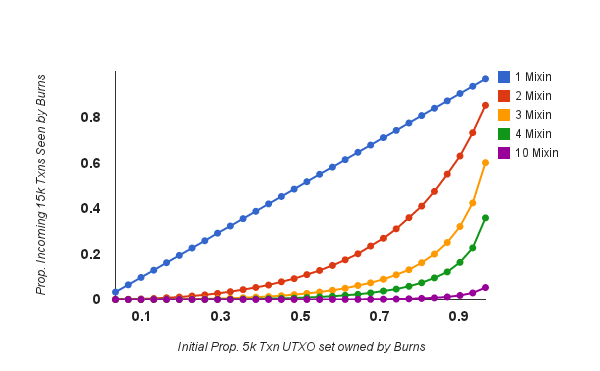
\includegraphics[width=0.95\textwidth,height=0.95\textheight,keepaspectratio]{burns.png}
\caption{This figure displays, with apologies to the color blind, the ``success of an attack'' executed by Burns. We see that, for increasing numbers of mixins, success uniformly decreases accross the board. To refresh the reader who probably jumped directly to this graph,  here's the scenario: Evil guy Burns starts with an initial proportion ($x$-axis) of the UTXO set, which has $5000$ transaction outputs inside of it. Then, a flood of $15,000$ new honest transactions hits the network, from Lisa to Milhouse and from Homer to Marge and so on, causing the UTXO set to quadruple in size. After this event, Burns could spend his initial proportion $P_I$ of the UTXO set with no mixins and consequently break the untraceability of a proportion of the $15,000$ ostensibly honest transactions. We display this proportion $\widehat{P}_F$ as a function of $P_I$. For $10$ mixins, Burns requires $55\%$ of the UTXO set to capture any of a quadrupling event at all, and requires $87\%$ of the UTXO set in order to capture even $1\%$ of a quadrupling event with these parameters.}
\label{fig1}
\end{figure}

It's clear that $\widehat{P}_F$ is monotonically increasing as a function of $P_0 = N_B/(N_B + N_W)$, but that the situation improves for greater numbers of ring signatures. Notice that there are some dynamical systems problems built into our data. If you graph $P_F$ vs. $P_I$, (rather than our $\widehat{P}_F$ vs. $P_I$) then you can interpret this as a discrete-time dynamical system's evolution function to see that Burns' share must go to zero over time for any mixin $\geq 2$. We can expect, in the $1$ mixin scenario, for the urn to stochastically jump up and down the $y=x$ line without appreciably, in expectation, moving in any direction in a random walk. However, as long as we require $M \geq 2$ mixins, any chain reaction will burn itself out, so to speak; Burns' share of the UTXO set will shrink to zero over time unless he takes action. Our results suggest that any mandatory mixin $\geq 2$ will allow the system to recover from a passive attack quite quickly. The code we used to generate data can probably be improved, but is located at \texttt{http://goo.gl/dGj5TZ} and we used Google Documents to generate figures.

\section{Critical Mass, Slow Chain Reactions, Active Attackers: Further Questions}

Recall that we set out to ask the question ``can a critical chain reaction occur?'' and the related question ``what network parameters can we choose to ensure that any plausible chain reaction burns itself out?'' So, what do we need for a critical mass? Consider the urn problem again. What happens to the composition of the urn as this game evolves, as we toss new black or white marbles into the urn as we draw more? Remember, black marbles are the ones that will be revealed; if we draw all black marbles, that means the next marble we add to the urn must be black. A critical mass scenario is one in which, if there are enough black marbles in the urn, then Burns starts grabbing more and more and more black marbles. If ever $P_F > P_I$, we could expect some sort of critical mass, but this does not occur. Except in numerical edge cases, $P_F \leq P_I$. With $2$ and more mixins, our chain reactions become truncated very rapidly.

Chain reactions act slower and slower as mixins increase. Thus, a single mixin is inappropriate for any currency problem, because an anonymous, malicious user may spam the network with transactions they control in the hopes that they eventually control greater proportions of the UTXO set. This would essentially make all transactions \emph{from then on} fully traceable (at least from Burns' point of view), and Burns doesn't have to take a single action after his initial seed transactions are planted in the UTXO set. This \emph{fixed initial cost} for the attacker leading to a never-ending stream of information in the form of traceable transactions from other users is, clearly, a catastrophic economic failure. This is so important, we are putting it in italics: \emph{any CryptoNote coin that allows for only $1$ mixin is vulnerable to a slow chain reaction in which the owner of very few private keys can violate the untraceability of much larger number of other users.} Requiring a mixin of at least $2$ for all transactions save for transactions that are willfully spent with $0$ mixins will keep these chain reactions, probabilistically, to a smaller length. Indeed, any number greater than $1$ will do, to force these chain reactions to burn themselves out, rather than to spread to the whole network, and the higher the better. Of course, a protocol-enforced, network-wide mandatory minimimum mixin of $M=10$ would, presumably, cause a blockchain bloat, which can hinder adoption, which has it's own security benefits in terms of network size. Hence, there is likely some optimal size of mandatory minimum mixin. We do no more than to suggest $M=2$ as a protocol-enforced mandatory minimum, and to advise users to use as many mixin signatures as their little hearts desire.

Note that our scenario might be different if we change parameters of our model, or if we change our assumptions to include active attackers. Let's discuss parameters real quick. We can consider the addition of each new marble as nudging Burns' \emph{passive} ownership probability one way or another. Unless Burns grabs almost all incoming transactions, his share of the UTXO set will be depleted over time. How do our parameters change this process? Recall that our parameters are:
\begin{enumerate}
\item $N_{B_0} = $ Number of initial atomic units controlled by Burns in UTXO set,
\item $N_{W_0} = $ the remaining atomic units in the UTXO set, and
\item $M = $ mandatory minimum mixin enforced by network protocol.
\end{enumerate}
However, we are really interested in $P_I = N_{B_0}/(N_{B_0} + N_{W_0})$ and $N_0 = N_{B_0} + N_{W_0}$. We have seen above how $P_I$ and $M$, in general, change the outcome of the experiment. As $N_0$ gets big, Burns' share will start to slow down. Meaning even if Burns is grabbing all of the incoming transactions, he's getting a reduced rate of returns in terms of overall proportion of the UTXO set that he owns. We can think of the UTXO set size as a mass. As it gets bigger, it gets harder to change its state. 

Another ``hidden'' parameter here is ``how many new transactions are being added?'' We swept this under the rug by simply saying ``okay, the UTXO set is going to quadruple from it's initial size,'' reducing our parameter space a little bit, and in so doing, we have reduced the importance of $N_0$ as a parameter. Indeed, we know how $N$ changes, so we can easily compute slope of any statistic, $T(N)$, with respect to ``change in population size'' and call that the sensitivity:
\[S = \frac{T(N_f) - T(N_o)}{N_f - N_o} = \frac{T(4\cdot N_o) - T(N_o)}{3N_o}\]
which, when close to zero, suggests no relationship, and when far from zero suggests a strong relationship (positive or negative). We could just as easily compute the slope of the log of the statistic with respect to the log of the population, and call that the sensitivity:
\[S = \frac{\log(T(N_f)) - \log(T(N_0))}{\log(N_f)-\log(N_o)} = \frac{1}{4}\log\left(\frac{T(4\cdot N_o)}{T(N_o)}\right)\]
in this version of sensitivity, we don't even see $N_f$ as part of the formula, simply the multiplicative factor $N_f/N_o = 4$. However, we feel it is unnecessary to present a full-scale parameter-space analysis of this model.

Now let's discuss changing assumptions. One apparently small tweak we could add to this simulation is to change assumption (iv). In order to model a more aggressive attacker rather than a ``Christmas Day'' accidental reveal sort of attack, we could implement a probabilistic assumption like
\begin{enumerate}[(v)]
\item Burns gains control of a new transaction as the result of a sequence of Bernoulli trials. With a fixed probability $q$, Burns generates a transaction that he knows is his, and with probability $1-q$, a foreign transaction appears and generates a new ring signature that may be solely composed with Burns-controlled transactions (i.e.\ Burns still participates in the economy)
\end{enumerate}
or we could implement a dynamical model where a malicious Burns tries to maintain a minimum proportion of the UTXO set by spamming transactions to the network whenever his proportion drops his secretly determined percentage:
\begin{enumerate}[(v)]
\item Burns gains control of a new transaction as the result of a sequence of non-autonomous, Bernoulli-like experiments. With a probability $q(B,N)$ dependent both on the number of UTXOs controlled by Burns, $B$, and the total UTXO set, $N$, Burns generates a transaction that he knows is his, and with probability $1-q(B,N)$, a foreign transaction appears and generates a new ring signature that may be solely composed with Burns controlled transactions.
\end{enumerate}
Any function $q(B,N)$ that Burns can try to make close to $1$ when $B/N$ is smaller than Burns' preference will allow Burns to grow his share of the UTXOset. Of course, the easiest, simplest strategy for Burns would be to just spam the network as fast as possible with his own transactions. But with fees, this isn't free. 

We bring up parameters and assumptions because the work is not really done on this problem. We have discovered what we, as network engineers, need to know in order to ensure graceful degradation: pick big mixins. However, there are really interesting questions still lurking under the surface. One of us solved this problem with graph theory, one of us with probability. Note that, as time goes on, a UTXO is more likely to be chosen for mixins, but is also more likely to have been exposed from previous users revealing their transactions by spending them with $0$ mixins, complicating the wisdom of choosing UTXOs for the ring signature from a uniform distribution. Technically, for any sort of ``critical mass'' sort of problem, there's going to be a steady state problem lurking under the surface, and we definitely have some dynamical systems stuff flying\footnote{See what I did there?} about in this problem.  Maybe some ambitious undergraduate wants to pick up where we leave off and contribute to the cryptocurrency community by expanding on all of this.

\begin{backmatter}
\end{backmatter}
\end{document}
